\documentclass{article}
\usepackage{tikz}
	
\begin{document}
	The curve below has been generated with the result of
	
	\verb+python3 krampouezh.py -tpgf cubic "(0,0)" "(5,2)" "(7,1)" "(10,0)"+
	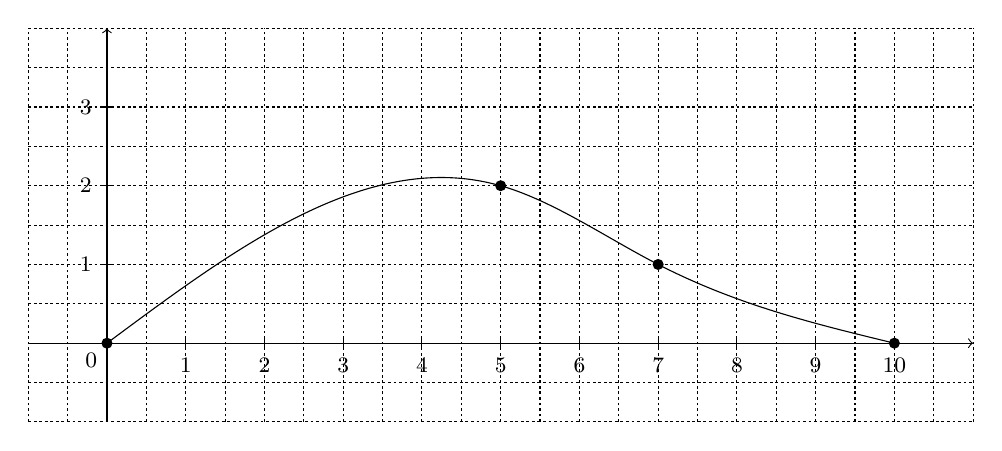
\begin{tikzpicture}
		\draw [color=black,dash pattern=on 1pt off 1pt, xstep=0.5cm,ystep=0.5cm] (-1,-1) grid (11,4);
		\draw[->] (-1,0) -- (11,0);
		\foreach \x in {1,2,3,4,5,6,7,8,9,10}
			\draw[shift={(\x,0)},color=black] (0pt,2pt) -- (0pt,-2pt) node[below] {\footnotesize $\x$};
		\draw[->,color=black] (0,-1) -- (0,4);
		\foreach \y in {1,2,3}
			\draw[shift={(0,\y)},color=black] (2pt,0pt) -- (-2pt,0pt) node[left] {\footnotesize $\y$};
		\draw[color=black] (0,0) node[below left] {\footnotesize $0$};
		\foreach \P in {{(0,0)}, {(5,2)}, {(7,1)}, {(10,0)}}
			\fill \P circle[radius=2pt];
		\draw[smooth,samples=100,domain=0.0:10.0] plot(\x,{((((0.0*((\x+(-0.0))^0))+(0.7431372549019608*((\x+(-0.0))^1))+(0.0*((\x+(-0.0))^2))+(-0.013725490196078433*((\x+(-0.0))^3)))*and(\x>=0.0,\x<5.0))+(((2.0*((\x+(-5.0))^0))+(-0.28627450980392155*((\x+(-5.0))^1))+(-0.2058823529411765*((\x+(-5.0))^2))+(0.04950980392156864*((\x+(-5.0))^3)))*and(\x>=5.0,\x<7.0))+(((1.0*((\x+(-7.0))^0))+(-0.515686274509804*((\x+(-7.0))^1))+(0.0911764705882353*((\x+(-7.0))^2))+(-0.010130718954248366*((\x+(-7.0))^3)))*and(\x>=7.0,\x<10.0)))});
	\end{tikzpicture}
\end{document}
